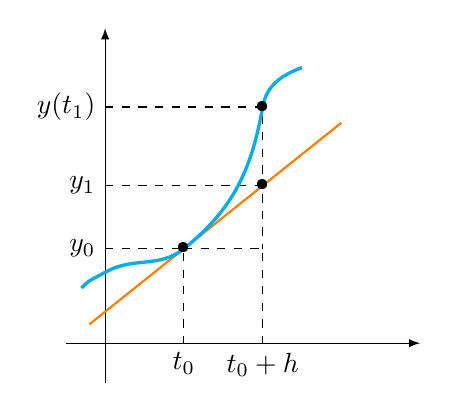
\begin{tikzpicture}[x=1cm,y=1cm]\centering
    \draw[-latex] (-0.5,0)--(4,0); % eixo x
    \draw[-latex] (0,-0.5)--(0,4); % eixo y

    \draw[dashed] (0,1.2) node[left] {$y_0$}--(1,1.2)--(1,0) node[below] {$t_0$}; % y0 -- * -- t0
    \draw[dashed] (1,1.2)--(2,1.2)--(2,0) node[below] {$t_0+h$}; % * -- * -- t_1 = t0+h
    \draw[dashed] (0,2) node[left] {$y_1$}--(2,2)--(2,1.2); % y1 -- * -- t_1 = t0+h
    \draw[dashed] (0,3) node[left] {$y(t_1)$}--(2,3)--(2,2); % y(t1) -- * -- *

    % reta passando pelos pontos (t0, y0) e (t0+h,y1)
    \draw[thick, orange] (-0.2,0.24) -- (3,2.8);

    % a curva
    \draw[very thick, cyan] (-0.3,0.7) 
    to[out=50,in=210] (0,0.9) 
    to[out=30,in=218.66] (1,1.2) 
    to[out=38.66,in=260] (2,3)
    to[out=80,in=200] (2.5,3.5);

    % pontos pretos (bullet)
    \foreach \Point in {(1,1.2),(2,2),(2,3)}{
        \node at \Point {\textbullet};
    }
\end{tikzpicture}